% Options for packages loaded elsewhere
\PassOptionsToPackage{unicode}{hyperref}
\PassOptionsToPackage{hyphens}{url}
%
\documentclass[
]{article}
\title{Métodos estadísticos aplicados al baloncesto}
\usepackage{etoolbox}
\makeatletter
\providecommand{\subtitle}[1]{% add subtitle to \maketitle
  \apptocmd{\@title}{\par {\large #1 \par}}{}{}
}
\makeatother
\subtitle{Trabajo Fin de Grado Estadística Apliacada}
\author{Paula Moreno}
\date{21/1/2022}

\usepackage{amsmath,amssymb}
\usepackage{lmodern}
\usepackage{iftex}
\ifPDFTeX
  \usepackage[T1]{fontenc}
  \usepackage[utf8]{inputenc}
  \usepackage{textcomp} % provide euro and other symbols
\else % if luatex or xetex
  \usepackage{unicode-math}
  \defaultfontfeatures{Scale=MatchLowercase}
  \defaultfontfeatures[\rmfamily]{Ligatures=TeX,Scale=1}
\fi
% Use upquote if available, for straight quotes in verbatim environments
\IfFileExists{upquote.sty}{\usepackage{upquote}}{}
\IfFileExists{microtype.sty}{% use microtype if available
  \usepackage[]{microtype}
  \UseMicrotypeSet[protrusion]{basicmath} % disable protrusion for tt fonts
}{}
\makeatletter
\@ifundefined{KOMAClassName}{% if non-KOMA class
  \IfFileExists{parskip.sty}{%
    \usepackage{parskip}
  }{% else
    \setlength{\parindent}{0pt}
    \setlength{\parskip}{6pt plus 2pt minus 1pt}}
}{% if KOMA class
  \KOMAoptions{parskip=half}}
\makeatother
\usepackage{xcolor}
\IfFileExists{xurl.sty}{\usepackage{xurl}}{} % add URL line breaks if available
\IfFileExists{bookmark.sty}{\usepackage{bookmark}}{\usepackage{hyperref}}
\hypersetup{
  pdftitle={Métodos estadísticos aplicados al baloncesto},
  pdfauthor={Paula Moreno},
  hidelinks,
  pdfcreator={LaTeX via pandoc}}
\urlstyle{same} % disable monospaced font for URLs
\usepackage[margin=1in]{geometry}
\usepackage{color}
\usepackage{fancyvrb}
\newcommand{\VerbBar}{|}
\newcommand{\VERB}{\Verb[commandchars=\\\{\}]}
\DefineVerbatimEnvironment{Highlighting}{Verbatim}{commandchars=\\\{\}}
% Add ',fontsize=\small' for more characters per line
\usepackage{framed}
\definecolor{shadecolor}{RGB}{248,248,248}
\newenvironment{Shaded}{\begin{snugshade}}{\end{snugshade}}
\newcommand{\AlertTok}[1]{\textcolor[rgb]{0.94,0.16,0.16}{#1}}
\newcommand{\AnnotationTok}[1]{\textcolor[rgb]{0.56,0.35,0.01}{\textbf{\textit{#1}}}}
\newcommand{\AttributeTok}[1]{\textcolor[rgb]{0.77,0.63,0.00}{#1}}
\newcommand{\BaseNTok}[1]{\textcolor[rgb]{0.00,0.00,0.81}{#1}}
\newcommand{\BuiltInTok}[1]{#1}
\newcommand{\CharTok}[1]{\textcolor[rgb]{0.31,0.60,0.02}{#1}}
\newcommand{\CommentTok}[1]{\textcolor[rgb]{0.56,0.35,0.01}{\textit{#1}}}
\newcommand{\CommentVarTok}[1]{\textcolor[rgb]{0.56,0.35,0.01}{\textbf{\textit{#1}}}}
\newcommand{\ConstantTok}[1]{\textcolor[rgb]{0.00,0.00,0.00}{#1}}
\newcommand{\ControlFlowTok}[1]{\textcolor[rgb]{0.13,0.29,0.53}{\textbf{#1}}}
\newcommand{\DataTypeTok}[1]{\textcolor[rgb]{0.13,0.29,0.53}{#1}}
\newcommand{\DecValTok}[1]{\textcolor[rgb]{0.00,0.00,0.81}{#1}}
\newcommand{\DocumentationTok}[1]{\textcolor[rgb]{0.56,0.35,0.01}{\textbf{\textit{#1}}}}
\newcommand{\ErrorTok}[1]{\textcolor[rgb]{0.64,0.00,0.00}{\textbf{#1}}}
\newcommand{\ExtensionTok}[1]{#1}
\newcommand{\FloatTok}[1]{\textcolor[rgb]{0.00,0.00,0.81}{#1}}
\newcommand{\FunctionTok}[1]{\textcolor[rgb]{0.00,0.00,0.00}{#1}}
\newcommand{\ImportTok}[1]{#1}
\newcommand{\InformationTok}[1]{\textcolor[rgb]{0.56,0.35,0.01}{\textbf{\textit{#1}}}}
\newcommand{\KeywordTok}[1]{\textcolor[rgb]{0.13,0.29,0.53}{\textbf{#1}}}
\newcommand{\NormalTok}[1]{#1}
\newcommand{\OperatorTok}[1]{\textcolor[rgb]{0.81,0.36,0.00}{\textbf{#1}}}
\newcommand{\OtherTok}[1]{\textcolor[rgb]{0.56,0.35,0.01}{#1}}
\newcommand{\PreprocessorTok}[1]{\textcolor[rgb]{0.56,0.35,0.01}{\textit{#1}}}
\newcommand{\RegionMarkerTok}[1]{#1}
\newcommand{\SpecialCharTok}[1]{\textcolor[rgb]{0.00,0.00,0.00}{#1}}
\newcommand{\SpecialStringTok}[1]{\textcolor[rgb]{0.31,0.60,0.02}{#1}}
\newcommand{\StringTok}[1]{\textcolor[rgb]{0.31,0.60,0.02}{#1}}
\newcommand{\VariableTok}[1]{\textcolor[rgb]{0.00,0.00,0.00}{#1}}
\newcommand{\VerbatimStringTok}[1]{\textcolor[rgb]{0.31,0.60,0.02}{#1}}
\newcommand{\WarningTok}[1]{\textcolor[rgb]{0.56,0.35,0.01}{\textbf{\textit{#1}}}}
\usepackage{graphicx}
\makeatletter
\def\maxwidth{\ifdim\Gin@nat@width>\linewidth\linewidth\else\Gin@nat@width\fi}
\def\maxheight{\ifdim\Gin@nat@height>\textheight\textheight\else\Gin@nat@height\fi}
\makeatother
% Scale images if necessary, so that they will not overflow the page
% margins by default, and it is still possible to overwrite the defaults
% using explicit options in \includegraphics[width, height, ...]{}
\setkeys{Gin}{width=\maxwidth,height=\maxheight,keepaspectratio}
% Set default figure placement to htbp
\makeatletter
\def\fps@figure{htbp}
\makeatother
\setlength{\emergencystretch}{3em} % prevent overfull lines
\providecommand{\tightlist}{%
  \setlength{\itemsep}{0pt}\setlength{\parskip}{0pt}}
\setcounter{secnumdepth}{-\maxdimen} % remove section numbering
\ifLuaTeX
  \usepackage{selnolig}  % disable illegal ligatures
\fi

\begin{document}
\maketitle

\hypertarget{abstract}{%
\section{Abstract}\label{abstract}}

Hoy en día, el deporte es un hobby muy popular por todo el mundo. Des de
pequeños, la gran mayoría de niños practican algún tipo de deporte,
especialmente aquellos que son de equipo. Eso nos lleva a querer saber
más del deporte, más detalles, más información. Nos entra la curiosidad
de ``¿quién es el mejor jugador?'', ``Qué equipo es mejor?'', o incluso
intentar prevenir qué equipo ganará según sus resultados anteriores. Y
gracias a los avances tecnológicos, cada vez se nos facilita más poder
seguir un deporte des de casa, ver la estadística de los deportistas e
incluso hay plataformas o juegos que nos permiten ser, de manera
virtual, managers de los clubs y, por lo tanto, nos facilitan mucha
información que antes era más difícil de saber.

Eso hace que, de manera progresiva, también mejore el estudio y el
análisis de cada deporte, y cada vez sea más específica para cada
deporte, implementando nuevos recursos para mejorar los resultados.

En este trabajo estudiaremos más a fondo el Baloncesto, el segundo
deporte más popular de Europa (solo superado por el futbol), y el cual
yo tengo relación personal, ya que lo practico des de los 4 años. En
especial nos centraremos en el Baloncesto profesional Europeo, de donde
podemos obtener más datos.

Este trabajo surgió del constante pensamiento de que los análisis
actuales que se hacen en este deporte en Europa son bastante pobres a
nivel informativo, puesto que se basan en conceptos muy básicos. Para
que nos hagamos una idea, el estadístico por preferencia es el llamado
``Valoración'' y que se originó en 1991 (hace 30 años) y des de entonces
nunca se ha modificado.

Es por eso que, considero que actualmente los análisis que se hacen de
este deporte necesitan una actualización para llegar a informar de todos
aquellos datos que hoy en día si se pueden recoger gracias a los avances
tecnológicos.

\hypertarget{contenido-borrador}{%
\section{Contenido (Borrador)}\label{contenido-borrador}}

\begin{enumerate}
\def\labelenumi{\arabic{enumi}.}
\setcounter{enumi}{-1}
\item
  Recursos informaticos nuevos que se han utilizado para hacer este
  trebajo: GitHub. Explicacion de qué es, como funciona y ventajas que
  tiene.
\item
  Introducción al baloncesto y breve explicación de cómo se juega
  (historia, conceptos importantes de conocer, y metodologia del juego)
\item
  Explicación de la Estadística Actual (formulas, definiciones)
\item
  Nuevos Analisis (breve explicacion de la nueva forma de recoger datos
  de los jugadores, y luego el mas/menos ajustado, Gini\ldots)
\item
  Analisis de los datos Temporada 2018-2019
\end{enumerate}

\hypertarget{recursos-informaticos}{%
\section{Recursos Informaticos}\label{recursos-informaticos}}

Para realizar este trabajo, mi tutor Sergio Olmos, me recomendó utilizar
GitHub porque era una manera de poder compartir mi proyecto de Markdown
con mis tutores de manera constante. Requería trabajar con el proyecto
publicado en dicha plataforma y de manera automática, cuando yo
modificara mi archivo, ellos podrían ver este cambio al momento. Yo
desconocía totalmente de este espacio, por lo que una parte de mi
trabajo era aprender a trabajar en GitHub.

\hypertarget{quuxe9-es-github}{%
\subsubsection{¿Qué es GitHub?}\label{quuxe9-es-github}}

GitHub es una plataforma de alojamiento, propiedad de Microsoft, que
ofrece a los desarrolladores la posibilidad de crear repositorios de
código y guardarlos en la nube de forma segura, usando un sistema de
control de versiones, llamado Git.

Como he comentado, facilita la organización de proyectos y permite la
colaboración de varios desarrolladores en tiempo real. Es decir, nos
permite centralizar el contenido del repositorio para poder colaborar
con los otros miembros de nuestro grupo des de varios dispositivos.

GitHub está basada en el sistema de control de versiones distribuida de
Git, por lo que se puede contar con sus funciones y herramientas, aunque
GitHub ofrece varias opciones adicionales y su interfaz es mucho más
fácil de manejar, por lo que no es absolutamente necesario que las
personas que lo utilizan tengan un gran conocimiento técnico.

\hypertarget{ventajas}{%
\subsubsection{Ventajas}\label{ventajas}}

Hay un gran número de razones por las que GitHub es una gran opción para
el control y gestión de proyectos de código. Como por ejemplo:

\begin{itemize}
\tightlist
\item
  GitHub permite que alojemos proyectos en repositorios de forma
  gratuita
\item
  Los repositorios son públicos por defecto. Sin embargo, GitHub te
  permite también alojar tus proyectos de manera privada
\item
  Puedes crear y compartir páginas web estáticas con GitHub Pages
\item
  Facilita compartir tus proyectos de una forma mucho más fácil y crear
  un portafolio
\item
  Te permite colaborar para mejorar los proyectos de otros y a otros
  mejorar o aportar a los tuyos
\item
  Ayuda reducir significativamente los errores humanos y escribir tu
  código más rápido con GitHub Copilot
\item
  Te da control de versiones, una herramienta muy útil.
\end{itemize}

\hypertarget{quuxe9-es-el-control-de-versiones}{%
\subsubsection{¿Qué es el control de
versiones?}\label{quuxe9-es-el-control-de-versiones}}

Se le llama control de versiones a la administración de los cambios que
se realizan sobre los elementos o la configuración de algún proyecto. En
otras palabras, el control de versiones sirve para conocer y autorizar
los cambios que realicen los colaboradores en tu proyecto, guardando
información extra de qué están incluyendo los cambios y cuándo se
hicieron. Este control comienza con una versión básica del documento y
luego va guardando los cambios que se hagan a lo largo del proyecto.

El control de versiones es una herramienta muy valiosa, pues con ella
puedes tener acceso a las versiones anteriores de tu proyecto si es que
en algún momento no llega a funcionar de forma correcta.

\hypertarget{quuxe9-es-git}{%
\subsubsection{¿Qué es Git?}\label{quuxe9-es-git}}

Git es un software de control de versiones diseñado por Linus Torvalds,
pensando en la eficiencia, la confiabilidad y compatibilidad del
mantenimiento de versiones de aplicaciones cuando estas tienen un gran
número de archivos de código fuente.

\hypertarget{diferencias-git-vs-github}{%
\paragraph{Diferencias Git vs GitHub}\label{diferencias-git-vs-github}}

Entonces, ¿qué diferencia Git de GitHub?. La principal diferencia es que
Git es un sistema que permite establecer un control de versiones,
mientras que GitHub es una plataforma que ofrece un grupo de funciones
que facilitan el uso de Git y la colaboración en tiempo real, así como
el almacenamiento en la nube.

\hypertarget{el-baloncesto}{%
\section{El baloncesto}\label{el-baloncesto}}

\hypertarget{historia-y-reglas-buxe1sicas}{%
\subsection{Historia y reglas
básicas}\label{historia-y-reglas-buxe1sicas}}

El baloncesto es un deporte de equipo que se originó en 1891, por James
Naismith, profesor de educación física en la escuela, que buscaba idear
un deporte que sus alumnos pudieran practicar bajo techo, pues los duros
inviernos en Nueva Inglaterra dificultaban la realización de ejercicio
al aire libre. Con el paso de los años, este deporte que empezó como
actividad de colegio, ha ido evolucionando mucho, añadiendo más reglas,
conceptos nuevos, límites de números de jugadores, se ha determinado
tiempos de juego, las canastas tienen un valor distinto según la
distancia, etc.

Actualmente, las normas más básicas de este deporte son:

\begin{itemize}
\tightlist
\item
  En las ligas superiores, hay un total de 4 cuartos de 10 minutos y
  pueden estar en pista 5 jugadores por equipo.
\item
  No te puedes desplazar con la pelota en las manos, es obligatorio
  botar con una mano (si no será una infracción y conllevará la perdida
  de pelota y saque de banda del equipo rival).
\item
  Cada jugador puede realizar hasta un total de 5 faltas, que será
  penalizado con un saque de banda o con un tiro libre (dependerá de la
  situación). El jugador que realiza 5 faltas será expulsado del
  partido.
\item
  El objetivo es encestar el máximo de puntos posibles, teniendo en
  cuenta que pueden sumar 1, 2 o 3 puntos, según la distancia.
\end{itemize}

\hypertarget{conceptos-y-definiciones-buxe1sicas-del-baloncesto}{%
\subsection{Conceptos y definiciones básicas del
baloncesto:}\label{conceptos-y-definiciones-buxe1sicas-del-baloncesto}}

Para que podamos entender a que nos referimos en este trabajo, es
necesario comprender unos conceptos básicos de vocabulario. Tendremos en
cuenta los conceptos que se necesitan para realizar la valoración del
jugador y/o del equipo que se utilizan en las estadísticas federadas.

\begin{itemize}
\tightlist
\item
  Puntos: Acumulación de canastas encestadas multiplicadas por su valor,
  que cada jugador y/o equipo realiza durante el partido
\item
  Minutos: Número de minutos que el jugador está en pista
\item
  Falta: Acción en la que un defensor bloquea el avance de su rival sin
  tener control de balón o de manera no reglamentaria (empujar,
  agarrar\ldots)
\item
  Perdidas de balón: cuando un equipo pierde el control del balón y pasa
  a ser del equipo rival.
\item
  Rebotes: Recuperación de pelota después de que el tiro sea ejecutado,
  pero no haya encestado.
\item
  Recuperación de balón: Cuando un equipo consigue robar el balón al
  equipo rival.
\item
  Asistencia: Es un pase a un jugador que se encuentra en una posición
  de ventaja o que le ayuda a conseguir una canasta sin hacer ningún
  bote.
\item
  Tapón: Bloqueo de un tiro en el aire.
\end{itemize}

\hypertarget{anuxe1lisis}{%
\subsection{Análisis}\label{anuxe1lisis}}

Viendo la gran cantidad de datos que se pueden extraer de cada partido
(y de cada equipo), se han ido creando análisis que recogen estos datos
y los analizan para ayudarnos a identificar y desarrollar hipótesis
sobre cada jugador y/o equipo.

\hypertarget{boxscore}{%
\subsection{Boxscore}\label{boxscore}}

El primer análisis que se hizo fue un \emph{Box Score} (Caja de
puntuación) donde se recopilaba únicamente los puntos de cada jugador
según el valor de esta y las faltas realizadas. Posteriormente, se fue
mejorando añadiendo conceptos como rebotes, tapones, perdidas de balón,
recuperaciones de balón\ldots{} Y se añadió el estadístico (que
acutalmente es por defecto) que se realiza a partir de todos estos
datos: ``Valoración'' (en inglés PIR, \emph{Performance Index Rating})
que engloba todo lo básico que pasa en el partido de manera individual y
que, cuanto más positivo, mejor. Este estadístico se calcula utilizando
la siguiente fórmula:

\[PIR = (Puntos + Rebotes + Asistencias + Robos + Tapones + Faltas Recibidas) - (Tiros de Campo Fallados + Tiros Libres Fallados + Tapones Recibidos + Pérdidas + Faltas Realizadas) \]

\begin{figure}
\centering
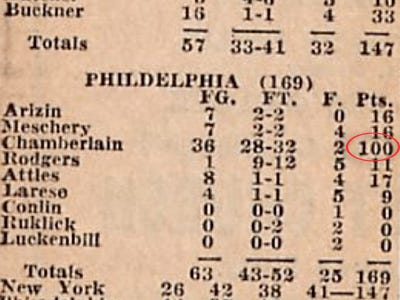
\includegraphics{imagenes/BoxScore1962.jpg}
\caption{Imagen 1. Boxscore del partido de la NBA de Philadelphia
Warriors contra New York Knicks, del 2 de Marzo de 1962}
\end{figure}

\begin{figure}
\centering
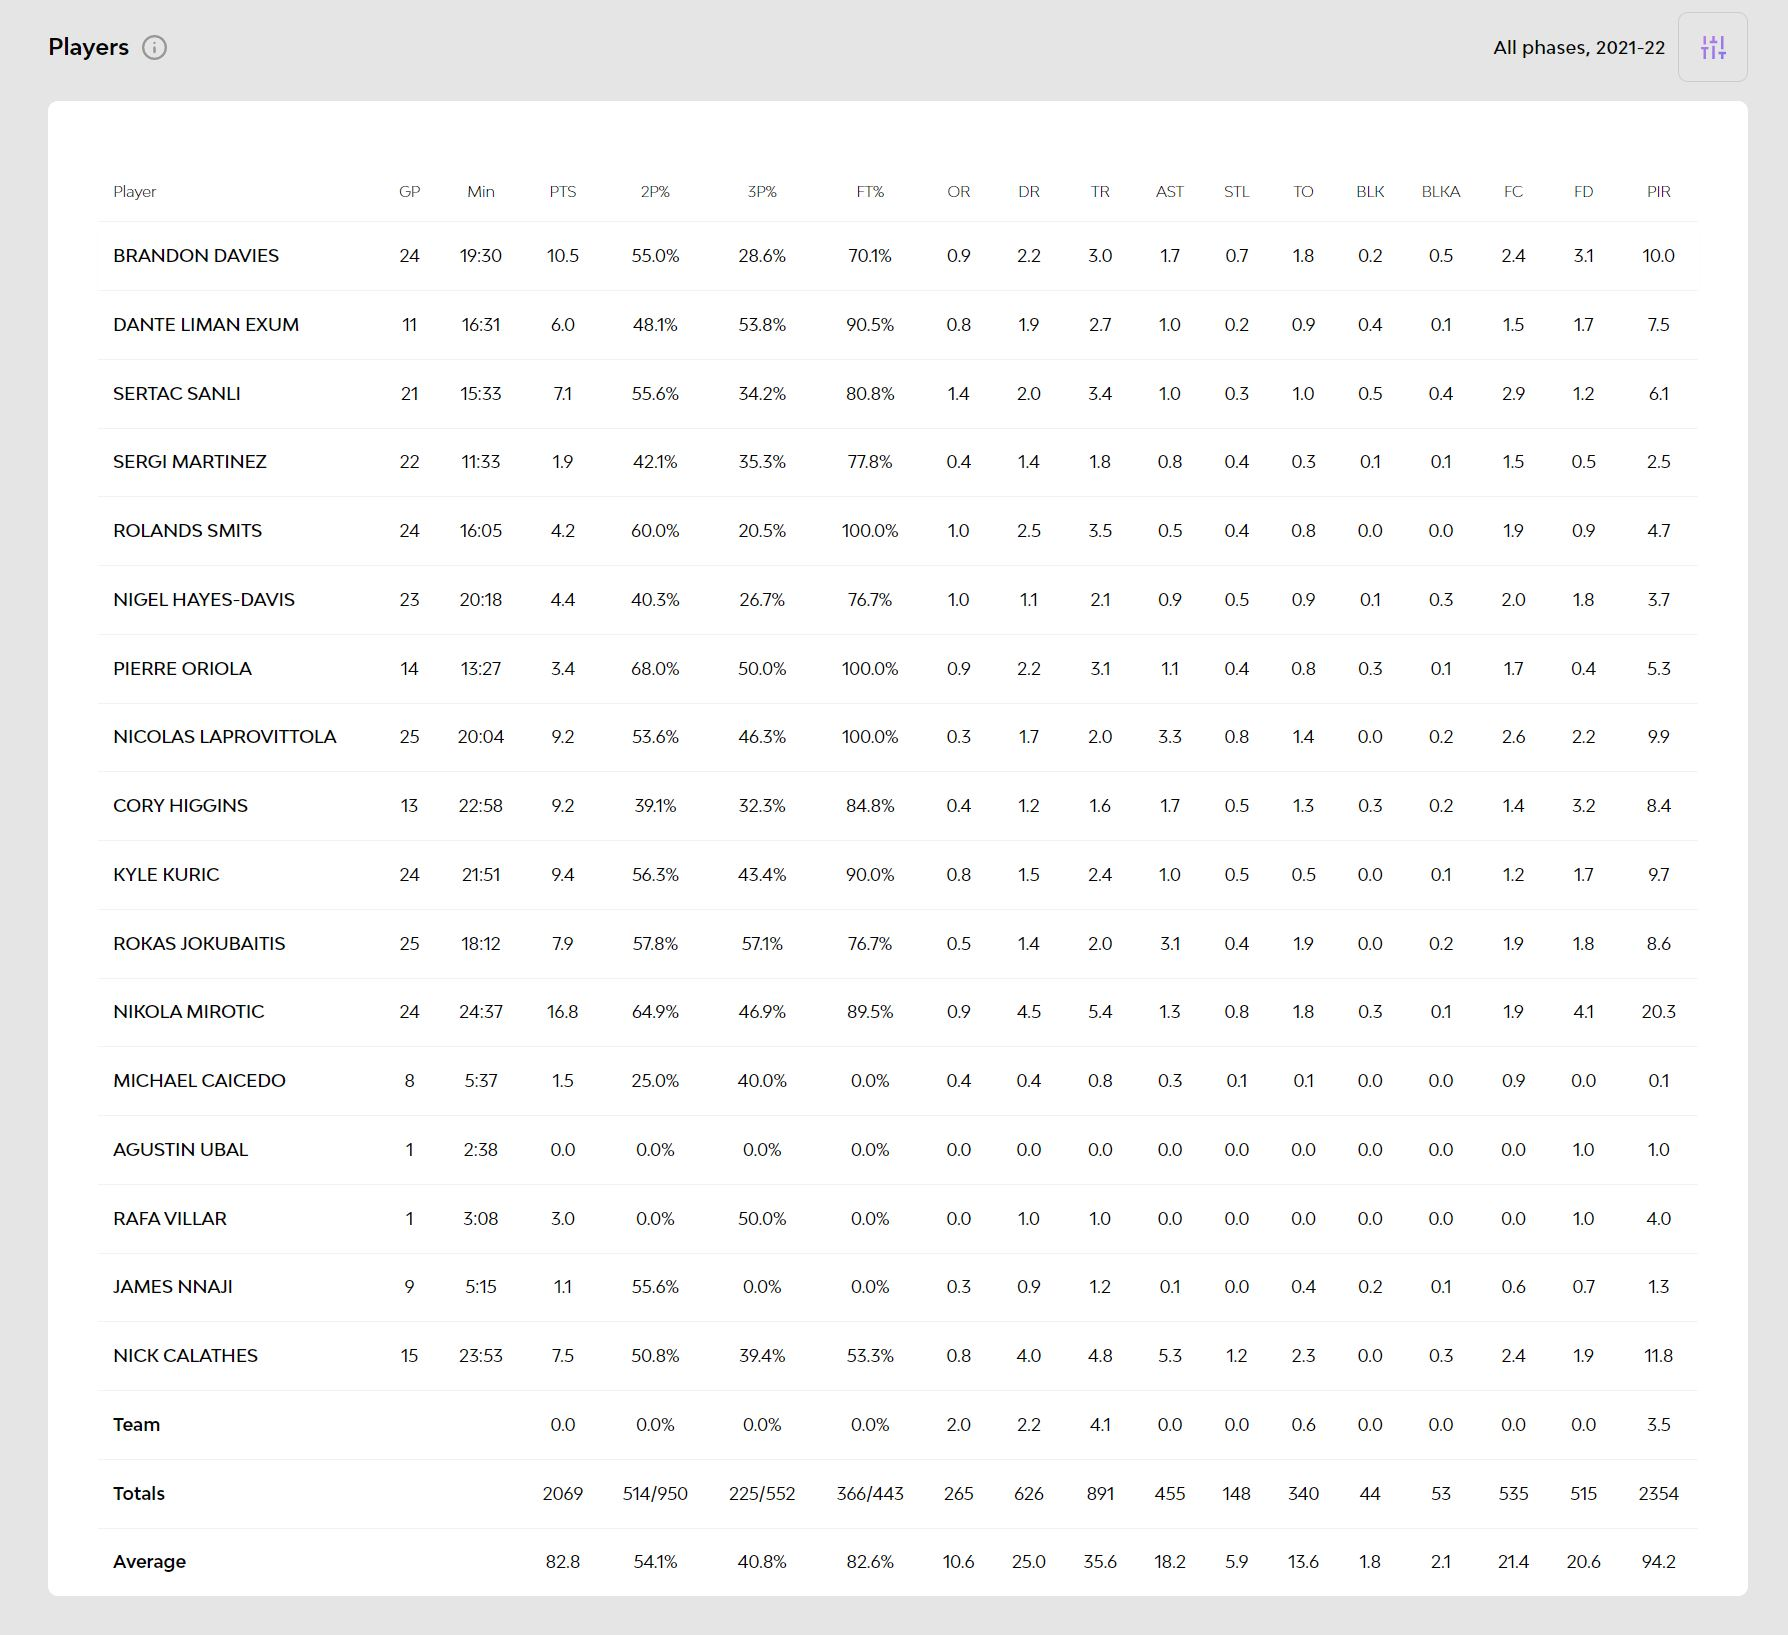
\includegraphics{imagenes/BoxScore2022_EuroligaBarca.JPG}
\caption{Imagen 2. Boxscore del partido de la Euroliga de Real Madrid
contra FC Barcelona, del 11 de Febrero del 2022}
\end{figure}

(en el
\protect\hyperlink{Anexo-1:-Descripciuxf3n-de-las-variables}{Anexo 1}
encontraréis la descripción de cada variable)

Posteriormente, se añadió la variable ``Más/Menos'' (P/M,
\emph{Plus/Minus}) que tiene que ver con la diferencia de puntos en el
marcador durante el tiempo que el jugador está en pista. Esta variable
sirve para ver la contribución de los jugadores cuando están en pista.
Todos los jugadores parten inicialmente con un 0, y según van entrando y
saliendo de la pista, esta variable se va actualizando. Por ejemplo, los
jugadores que son del quinteto inicial, empiezan con el marcador 0 - 0,
y un P/M = 0. Si en el minuto 5, se substituye un jugador en cancha del
equipo local (J1) por otro que está descansando (J2), y el marcador va
12 - 7, el P/M del J1 pasará a ser +5. Y si al cabo de 3 minutos, se
sustituye el J2 por otro (J3) y el marcador ahora va 20 - 9, el P/M del
J2 será +6 (\$ (20-12) - (9-7) = 8 - 2 = +6 \$).

Aunque un \emph{Box Score} es muy útil para realizar análisis básicos,
ya que es muy visual y cualquier persona sin la necesidad de muchos
recursos puede analizar y predecir ciertos valores, pero
estadísticamente perdemos una parte importante de la información de los
datos, puesto que no nos los muestra progresivamente, sino que nos da
los valores acumulados al final del tiempo establecido, y muchas veces
contiene información engañosa, especialmente en las estadísticas
defensivas.

Por lo que, para el desarrollo temporal del partido y para conocer
cierta información de equipo que piden entrenadores y clubs, no nos
sirve (como por ejemplo la eficacia de los quintetos, el desarrollo del
marcador o de cualquier otra variable del equipo entero durante un
tiempo determinado del partido, etc.)

\hypertarget{play-by-play}{%
\subsection{play-by-play}\label{play-by-play}}

Este tipo de recogida de información se creo para solucionar el problema
que teniamos con el \emph{Box Score}. Los datos de \emph{Play-by-Play}
(PBP) han sido la fuente principal de muchas estadísticas avanzadas,
como el más-menos ajustado, que se desarrollará en este trabajo.

\emph{Play-by-Play} proporciona una transcripción del juego en un
formato de eventos individuales. Los datos típicos de jugada por jugada
deben tener la siguiente información: - El tiempo de la posesión - El
jugador que inició la posesión (en caso de robo o rebote defensivo) - El
jugador contrario que inició la posesión (en caso de un tiro fallado o
pérdida de balón), incluida la ubicación en el piso desde donde se
realizó el tiro y algunos otros identificadores únicos que usamos para
clasificar el tipo de posesión.

\hypertarget{shot-charts}{%
\subsection{shot-charts}\label{shot-charts}}

\begin{center}\rule{0.5\linewidth}{0.5pt}\end{center}

\hypertarget{bibliografia}{%
\section{Bibliografia}\label{bibliografia}}

Sport in Europe (Wikipedia):
\url{https://en.wikipedia.org/wiki/Sport_in_Europe}

Valoración (Wikipedia):
\url{https://en.wikipedia.org/wiki/Performance_Index_Rating}

Git (Wikipedia): \url{https://es.wikipedia.org/wiki/Git}

GitHub (Wikipedia): \url{https://es.wikipedia.org/wiki/GitHub}

Baloncesto (Wikipedia): \url{https://es.wikipedia.org/wiki/Baloncesto}

Valoración (Wikipedia):
\url{https://es.wikipedia.org/wiki/Valoraci\%C3\%B3n_(baloncesto)}

\hypertarget{anexo-1-descripciuxf3n-de-las-variables}{%
\section{Anexo 1: Descripción de las
variables}\label{anexo-1-descripciuxf3n-de-las-variables}}

\begin{itemize}
\tightlist
\item
  MIN (\emph{Minutes}): Minutos totales jugados
\item
  PTS (\emph{points}): Puntos totales realizados
\item
  2FGA (\emph{2-point Field Goals Attempted}): Número de canastas de 2
  puntos intentadas
\item
  2FGM (\emph{2-point Field Goals Made}): Número de canastas de 2 puntos
  anotadas
\item
  3FGA (\emph{3-point Field Goals Attempted}): Número de canastas de 3
  puntos (``triples'') intentadas
\item
  3FGM (\emph{3-point Field Goals Made}): Número de canastas de 3 puntos
  (``triples'') anotadas
\item
  FTA (\emph{Free Throws Attempted}): Número de tiros libres intentados
\item
  FTM (\emph{Free Throws Made}): Número de tiros libres anotados
\end{itemize}

\begin{center}\rule{0.5\linewidth}{0.5pt}\end{center}

\hypertarget{datos}{%
\section{Datos}\label{datos}}

\begin{Shaded}
\begin{Highlighting}[]
\FunctionTok{library}\NormalTok{(readr)}
\NormalTok{pbp2018 }\OtherTok{\textless{}{-}} \FunctionTok{read.csv}\NormalTok{(}\AttributeTok{file=}\StringTok{"pbp2018.csv"}\NormalTok{, }\AttributeTok{head=}\ConstantTok{TRUE}\NormalTok{, }\AttributeTok{sep=}\StringTok{","}\NormalTok{)}
\CommentTok{\#View(pbp2018)}
\end{Highlighting}
\end{Shaded}

\hypertarget{paquetes}{%
\subsubsection{Paquetes}\label{paquetes}}

\begin{Shaded}
\begin{Highlighting}[]
\FunctionTok{library}\NormalTok{(dplyr)}
\FunctionTok{library}\NormalTok{(ggplot2)}
\end{Highlighting}
\end{Shaded}

\hypertarget{cp---areglarlo}{%
\paragraph{CP - Areglarlo!}\label{cp---areglarlo}}

\hypertarget{alineaciones-con-jugadores-repetidos}{%
\subsubsection{Alineaciones con jugadores
repetidos}\label{alineaciones-con-jugadores-repetidos}}

\hypertarget{paquetes-1}{%
\subsection{Paquetes}\label{paquetes-1}}

\begin{Shaded}
\begin{Highlighting}[]
\FunctionTok{library}\NormalTok{(here)}
\FunctionTok{library}\NormalTok{(tidyverse)}
\end{Highlighting}
\end{Shaded}

\hypertarget{problema}{%
\subsection{Problema}\label{problema}}

Algunos registros en \texttt{pbp\_2018.csv} contenían alineaciones con
un mismo jugador que aperece dos veces.

Tras inspeccionar la función del paquete eurolig que obtiene las
alineaciones de estos datos, descubrí que se trataba de un error en la
función que asigna las alineaciones en las situaciones en las que hay
cambios de jugadores cuando hay tiros libres. Solo afectaba a las
variables \texttt{away\_player4} y \texttt{away\_player5}.

\begin{Shaded}
\begin{Highlighting}[]
\NormalTok{pbp\_2018 }\OtherTok{\textless{}{-}} \FunctionTok{read\_csv}\NormalTok{(}\StringTok{"pbp2018.csv"}\NormalTok{)}
\end{Highlighting}
\end{Shaded}

\begin{verbatim}
## Warning: One or more parsing issues, see `problems()` for details
\end{verbatim}

\begin{Shaded}
\begin{Highlighting}[]
\DocumentationTok{\#\# Check how many rows are affected by this}
\NormalTok{bad\_lineups }\OtherTok{\textless{}{-}}\NormalTok{ pbp\_2018 }\SpecialCharTok{\%\textgreater{}\%}
  \FunctionTok{select}\NormalTok{(}\FunctionTok{matches}\NormalTok{(}\StringTok{"\_player[1{-}5]"}\NormalTok{)) }\SpecialCharTok{\%\textgreater{}\%}
  \FunctionTok{apply}\NormalTok{(}\DecValTok{1}\NormalTok{, }\ControlFlowTok{function}\NormalTok{(x) }\FunctionTok{max}\NormalTok{(}\FunctionTok{table}\NormalTok{(x)) }\SpecialCharTok{\textgreater{}} \DecValTok{1}\NormalTok{)}
\NormalTok{pbp\_bad }\OtherTok{\textless{}{-}}\NormalTok{ pbp\_2018 }\SpecialCharTok{\%\textgreater{}\%}
  \FunctionTok{filter}\NormalTok{(bad\_lineups)}
\NormalTok{pbp\_bad }\SpecialCharTok{\%\textgreater{}\%}
  \FunctionTok{select}\NormalTok{(season, game\_code, play\_number, play\_type, away\_player4, away\_player5)}
\end{Highlighting}
\end{Shaded}

\begin{verbatim}
## # A tibble: 10,260 x 6
##    season game_code play_number play_type away_player4 away_player5
##     <dbl>     <dbl>       <dbl> <chr>     <chr>        <chr>       
##  1   2018         2          93 IN        TOMIC, ANTE  TOMIC, ANTE 
##  2   2018         2          94 OUT       TOMIC, ANTE  TOMIC, ANTE 
##  3   2018         2          95 OUT       TOMIC, ANTE  TOMIC, ANTE 
##  4   2018         2          96 IN        TOMIC, ANTE  TOMIC, ANTE 
##  5   2018         2          97 OUT       TOMIC, ANTE  TOMIC, ANTE 
##  6   2018         2          98 IN        TOMIC, ANTE  TOMIC, ANTE 
##  7   2018         2          99 OUT       TOMIC, ANTE  TOMIC, ANTE 
##  8   2018         2         100 FTM       TOMIC, ANTE  TOMIC, ANTE 
##  9   2018         2         101 FTM       TOMIC, ANTE  TOMIC, ANTE 
## 10   2018         2         116 AST       KURIC, KYLE  KURIC, KYLE 
## # ... with 10,250 more rows
\end{verbatim}

\hypertarget{soluciuxf3n}{%
\subsection{Solución}\label{soluciuxf3n}}

He creado unas funciones en \href{fix-lineups.R}{\texttt{fix-lineups.R}}
para corregir este error en los datos que ya tenemos.

\begin{Shaded}
\begin{Highlighting}[]
\FunctionTok{source}\NormalTok{(}\FunctionTok{here}\NormalTok{(}\StringTok{"R"}\NormalTok{, }\StringTok{"fix{-}lineups.R"}\NormalTok{))}
\DocumentationTok{\#\# Function fix\_lineups() only takes data from a single game,}
\DocumentationTok{\#\# so I split the data and apply the function to each splitted data frame.}
\NormalTok{pbp\_2018\_fixed }\OtherTok{\textless{}{-}} \FunctionTok{split}\NormalTok{(pbp\_2018, }\FunctionTok{factor}\NormalTok{(pbp\_2018}\SpecialCharTok{$}\NormalTok{game\_code)) }\SpecialCharTok{\%\textgreater{}\%}
  \FunctionTok{map\_df}\NormalTok{(fix\_lineups)}
\DocumentationTok{\#\# Check that this has been fixed}
\NormalTok{pbp\_2018\_fixed }\SpecialCharTok{\%\textgreater{}\%}
  \FunctionTok{select}\NormalTok{(}\FunctionTok{matches}\NormalTok{(}\StringTok{"\_player[1{-}5]"}\NormalTok{)) }\SpecialCharTok{\%\textgreater{}\%}
  \FunctionTok{apply}\NormalTok{(}\DecValTok{1}\NormalTok{, }\ControlFlowTok{function}\NormalTok{(x) }\FunctionTok{max}\NormalTok{(}\FunctionTok{table}\NormalTok{(x)) }\SpecialCharTok{\textgreater{}} \DecValTok{1}\NormalTok{) }\SpecialCharTok{\%\textgreater{}\%}
  \FunctionTok{sum}\NormalTok{()}
\end{Highlighting}
\end{Shaded}

\begin{verbatim}
## [1] 0
\end{verbatim}

Finalmente escribo los datos corregidos en
\texttt{data/pbp\_2018\_fixed.csv}.

\begin{Shaded}
\begin{Highlighting}[]
\CommentTok{\#write\_csv(pbp\_2018\_fixed, here("data", "pbp\_2018\_fixed.csv"))}

\CommentTok{\#pbp2018\_f \textless{}{-} read.csv(file="pbp\_2018\_fixed.csv", head=TRUE, sep=",")}
\CommentTok{\#View(pbp2018\_f)}
\end{Highlighting}
\end{Shaded}

\begin{center}\rule{0.5\linewidth}{0.5pt}\end{center}

\hypertarget{masmenos}{%
\section{MAS/MENOS}\label{masmenos}}

\hypertarget{masmenos-ajustado-season-2018}{%
\section{MAS/MENOS AJUSTADO (season
2018)}\label{masmenos-ajustado-season-2018}}

\begin{Shaded}
\begin{Highlighting}[]
\CommentTok{\# Lista de jugadores:}
\NormalTok{players\_rep }\OtherTok{\textless{}{-}}\NormalTok{ pbp\_2018\_fixed}\SpecialCharTok{$}\NormalTok{player\_name}
\NormalTok{players }\OtherTok{\textless{}{-}} \FunctionTok{unique}\NormalTok{(players\_rep)}
\end{Highlighting}
\end{Shaded}

EXPLICAR BIEN TODOS LOS DATOS (los utilizados almenos)!!!

\begin{Shaded}
\begin{Highlighting}[]
\CommentTok{\# Matriz Stint y vectores respuesta:}
\NormalTok{stints }\OtherTok{\textless{}{-}} \FunctionTok{as.data.frame}\NormalTok{(}\FunctionTok{matrix}\NormalTok{( ,}\DecValTok{0}\NormalTok{,}\FunctionTok{length}\NormalTok{(players)))}
\FunctionTok{names}\NormalTok{(stints) }\OtherTok{\textless{}{-}}\NormalTok{ players}
\NormalTok{stintCount }\OtherTok{=} \DecValTok{1}

\CommentTok{\# Acciones que termina una posesion de pelota:}
\DocumentationTok{\#\# Canastas encestada (2/3/tiro libre), rebote defensivo, pelota recuperada}
\NormalTok{shots }\OtherTok{\textless{}{-}}\NormalTok{ pbp\_2018\_fixed[}\FunctionTok{which}\NormalTok{(pbp\_2018\_fixed}\SpecialCharTok{$}\NormalTok{play\_type }\SpecialCharTok{==} \StringTok{"2FGM"} \SpecialCharTok{|}\NormalTok{ pbp\_2018\_fixed}\SpecialCharTok{$}\NormalTok{play\_type }\SpecialCharTok{==} \StringTok{"3FGM"} \SpecialCharTok{|}\NormalTok{ pbp\_2018\_fixed}\SpecialCharTok{$}\NormalTok{play\_type }\SpecialCharTok{==} \StringTok{"FTM"} \SpecialCharTok{|}\NormalTok{ pbp\_2018\_fixed}\SpecialCharTok{$}\NormalTok{play\_type }\SpecialCharTok{==} \StringTok{"DRB"} \SpecialCharTok{|}\NormalTok{ pbp\_2018\_fixed}\SpecialCharTok{$}\NormalTok{play\_type }\SpecialCharTok{==} \StringTok{"TOV"}\NormalTok{),]}

\CommentTok{\#View(shots)}
\NormalTok{num\_shots }\OtherTok{\textless{}{-}} \FunctionTok{dim}\NormalTok{(shots)[}\DecValTok{1}\NormalTok{]}

\NormalTok{shots}\SpecialCharTok{$}\NormalTok{points }\OtherTok{=} \DecValTok{0}
\ControlFlowTok{for}\NormalTok{(i }\ControlFlowTok{in} \DecValTok{1}\SpecialCharTok{:}\NormalTok{num\_shots)\{}
  \ControlFlowTok{if}\NormalTok{(shots}\SpecialCharTok{$}\NormalTok{play\_type[i] }\SpecialCharTok{==} \StringTok{"2FGM"}\NormalTok{) shots}\SpecialCharTok{$}\NormalTok{points[i]}\OtherTok{=}\DecValTok{2}
  \ControlFlowTok{if}\NormalTok{(shots}\SpecialCharTok{$}\NormalTok{play\_type[i] }\SpecialCharTok{==} \StringTok{"3FGM"}\NormalTok{) shots}\SpecialCharTok{$}\NormalTok{points[i]}\OtherTok{=}\DecValTok{3}
  \ControlFlowTok{if}\NormalTok{(shots}\SpecialCharTok{$}\NormalTok{play\_type[i] }\SpecialCharTok{==} \StringTok{"FTM"}\NormalTok{) shots}\SpecialCharTok{$}\NormalTok{points[i]}\OtherTok{=}\DecValTok{1}
\NormalTok{\}}

\NormalTok{awayplayersStart }\OtherTok{\textless{}{-}} \FunctionTok{levels}\NormalTok{(}\FunctionTok{droplevels}\NormalTok{(}\FunctionTok{as.factor}\NormalTok{(}\FunctionTok{unique}\NormalTok{(}\FunctionTok{unlist}\NormalTok{(shots[}\DecValTok{30}\NormalTok{,}\DecValTok{24}\SpecialCharTok{:}\DecValTok{28}\NormalTok{])))))}
\NormalTok{homeplayersStart }\OtherTok{\textless{}{-}} \FunctionTok{levels}\NormalTok{(}\FunctionTok{droplevels}\NormalTok{(}\FunctionTok{as.factor}\NormalTok{(}\FunctionTok{unique}\NormalTok{(}\FunctionTok{unlist}\NormalTok{(shots[}\DecValTok{1}\NormalTok{,}\DecValTok{19}\SpecialCharTok{:}\DecValTok{23}\NormalTok{])))))}

\NormalTok{awayplayers}\OtherTok{\textless{}{-}}\FunctionTok{matrix}\NormalTok{(,num\_shots,}\DecValTok{5}\NormalTok{)}
\NormalTok{homeplayers}\OtherTok{\textless{}{-}}\FunctionTok{matrix}\NormalTok{(,num\_shots,}\DecValTok{5}\NormalTok{)}

\ControlFlowTok{for}\NormalTok{ (i }\ControlFlowTok{in} \DecValTok{1}\SpecialCharTok{:}\NormalTok{num\_shots) \{}
\NormalTok{  awayplayers[i,] }\OtherTok{\textless{}{-}} \FunctionTok{levels}\NormalTok{(}\FunctionTok{droplevels}\NormalTok{(}\FunctionTok{as.factor}\NormalTok{(}\FunctionTok{unique}\NormalTok{(}\FunctionTok{unlist}\NormalTok{(shots[i,}\DecValTok{24}\SpecialCharTok{:}\DecValTok{28}\NormalTok{])))))}
\NormalTok{  homeplayers[i,] }\OtherTok{\textless{}{-}} \FunctionTok{levels}\NormalTok{(}\FunctionTok{droplevels}\NormalTok{(}\FunctionTok{as.factor}\NormalTok{(}\FunctionTok{unique}\NormalTok{(}\FunctionTok{unlist}\NormalTok{(shots[i,}\DecValTok{19}\SpecialCharTok{:}\DecValTok{23}\NormalTok{])))))}
\NormalTok{\}}

\CommentTok{\#View(awayplayers)}

\NormalTok{bothHome }\OtherTok{\textless{}{-}}\NormalTok{ homeplayersStart }\SpecialCharTok{\%in\%}\NormalTok{ homeplayers}
\NormalTok{bothAway }\OtherTok{\textless{}{-}}\NormalTok{ awayplayersStart }\SpecialCharTok{\%in\%}\NormalTok{ awayplayers}
\end{Highlighting}
\end{Shaded}

\begin{Shaded}
\begin{Highlighting}[]
\NormalTok{possessions}\OtherTok{=}\DecValTok{0}
\NormalTok{homeScore}\OtherTok{=}\DecValTok{0}
\NormalTok{homePoints}\OtherTok{=}\DecValTok{0}
\NormalTok{awayScore}\OtherTok{=}\DecValTok{0}
\NormalTok{awayPoint}\OtherTok{=}\DecValTok{0}

\ControlFlowTok{if}\NormalTok{(}\FunctionTok{all}\NormalTok{(bothHome) }\SpecialCharTok{==} \ConstantTok{TRUE} \SpecialCharTok{\&} \FunctionTok{all}\NormalTok{(bothAway)}\SpecialCharTok{==}\ConstantTok{TRUE}\NormalTok{)\{}
  
  \ControlFlowTok{for}\NormalTok{ (i }\ControlFlowTok{in} \DecValTok{1}\SpecialCharTok{:}\NormalTok{num\_shots) \{ }\CommentTok{\#num\_shots}
  \ControlFlowTok{if}\NormalTok{(shots[i,}\StringTok{\textquotesingle{}play\_type\textquotesingle{}}\NormalTok{] }\SpecialCharTok{==} \StringTok{"FTM"}\SpecialCharTok{|}\NormalTok{ shots[i,}\StringTok{\textquotesingle{}play\_type\textquotesingle{}}\NormalTok{] }\SpecialCharTok{==} \StringTok{"2FGM"}\SpecialCharTok{|}\NormalTok{ shots[i,}\StringTok{\textquotesingle{}play\_type\textquotesingle{}}\NormalTok{] }\SpecialCharTok{==} \StringTok{"3FGM"}\NormalTok{)\{}
\NormalTok{    possessions }\OtherTok{=}\NormalTok{ possessions }\SpecialCharTok{+} \DecValTok{1}
    
    \ControlFlowTok{if}\NormalTok{(awayScore }\SpecialCharTok{==}\NormalTok{ shots[i, }\StringTok{\textquotesingle{}points\_away\textquotesingle{}}\NormalTok{])\{}
      \CommentTok{\# Local }
\NormalTok{      homeScore }\OtherTok{=}\NormalTok{ homeScore }\SpecialCharTok{+}\NormalTok{ shots[i, }\StringTok{\textquotesingle{}points\textquotesingle{}}\NormalTok{]}
\NormalTok{      homePoints }\OtherTok{=}\NormalTok{ homePoints }\SpecialCharTok{+}\NormalTok{ shots[i, }\StringTok{\textquotesingle{}points\textquotesingle{}}\NormalTok{]}
\NormalTok{    \}}
    
\CommentTok{\#! No entiendo la diferencia entre estas dos variables... a parte, nosaltros ya la tenemos no? "points\_home" y "points\_away"}
    \ControlFlowTok{else}\NormalTok{\{}
      \CommentTok{\# Visitante}
\NormalTok{      awayScore }\OtherTok{=}\NormalTok{ awayScore }\SpecialCharTok{+}\NormalTok{ shots[i, }\StringTok{\textquotesingle{}points\textquotesingle{}}\NormalTok{]}
\NormalTok{      awayPoint }\OtherTok{=}\NormalTok{ awayPoint }\SpecialCharTok{+}\NormalTok{ shots[i, }\StringTok{\textquotesingle{}points\textquotesingle{}}\NormalTok{]}
      
      \CommentTok{\#print(c(awayScore, homeScore, shots[i,\textquotesingle{}points\_away\textquotesingle{}], shots[i,\textquotesingle{}points\_home\textquotesingle{}], possessions))}
\NormalTok{    \}}
\NormalTok{  \}}
  \ControlFlowTok{else} \ControlFlowTok{if}\NormalTok{(shots[i,}\StringTok{\textquotesingle{}play\_type\textquotesingle{}}\NormalTok{] }\SpecialCharTok{==} \StringTok{"DRB"}\NormalTok{)\{}
\NormalTok{    possessions}\OtherTok{=}\NormalTok{ possessions }\SpecialCharTok{+} \DecValTok{1}
\NormalTok{  \}}
  \ControlFlowTok{else} \ControlFlowTok{if}\NormalTok{(shots[i,}\StringTok{\textquotesingle{}play\_type\textquotesingle{}}\NormalTok{] }\SpecialCharTok{==} \StringTok{"TOV"}\NormalTok{)\{}
\NormalTok{    possessions}\OtherTok{=}\NormalTok{ possessions }\SpecialCharTok{+} \DecValTok{1}
\NormalTok{  \}}
\NormalTok{  \}}
\NormalTok{\}}
\end{Highlighting}
\end{Shaded}


\end{document}
